\documentclass[12pt,b5paper]{ltjsarticle}

%\usepackage[margin=15truemm, top=5truemm, bottom=5truemm]{geometry}
%\usepackage[margin=10truemm,left=15truemm]{geometry}
\usepackage[margin=10truemm]{geometry}

\usepackage{amsmath,amssymb}
%\pagestyle{headings}
\pagestyle{empty}

%\usepackage{listings,url}
%\renewcommand{\theenumi}{(\arabic{enumi})}

\usepackage{graphicx}

\usepackage{tikz}
%\usetikzlibrary {arrows.meta}
\usetikzlibrary{intersections,calc,arrows.meta}

%\usepackage{wrapfig}
%\usepackage{bm}

% ルビを振る
%\usepackage{luatexja-ruby}	% required for `\ruby'

%% 核Ker 像Im Hom を定義
%\newcommand{\Img}{\mathop{\mathrm{Im}}\nolimits}
%\newcommand{\Ker}{\mathop{\mathrm{Ker}}\nolimits}
%\newcommand{\Hom}{\mathop{\mathrm{Hom}}\nolimits}

%\DeclareMathOperator{\Rot}{rot}
%\DeclareMathOperator{\Div}{div}
%\DeclareMathOperator{\Grad}{grad}
%\DeclareMathOperator{\arcsinh}{arcsinh}
%\DeclareMathOperator{\arccosh}{arccosh}
%\DeclareMathOperator{\arctanh}{arctanh}



%\usepackage{listings,url}
%
%\lstset{
%%プログラム言語(複数の言語に対応,C,C++も可)
%  language = Python,
%%  language = Lisp,
%%  language = C,
%  %背景色と透過度
%  %backgroundcolor={\color[gray]{.90}},
%  %枠外に行った時の自動改行
%  breaklines = true,
%  %自動改行後のインデント量(デフォルトでは20[pt])
%  breakindent = 10pt,
%  %標準の書体
%%  basicstyle = \ttfamily\scriptsize,
%  basicstyle = \ttfamily,
%  %コメントの書体
%%  commentstyle = {\itshape \color[cmyk]{1,0.4,1,0}},
%  %関数名等の色の設定
%  classoffset = 0,
%  %キーワード(int, ifなど)の書体
%%  keywordstyle = {\bfseries \color[cmyk]{0,1,0,0}},
%  %表示する文字の書体
%  %stringstyle = {\ttfamily \color[rgb]{0,0,1}},
%  %枠 "t"は上に線を記載, "T"は上に二重線を記載
%  %他オプション:leftline,topline,bottomline,lines,single,shadowbox
%  frame = TBrl,
%  %frameまでの間隔(行番号とプログラムの間)
%  framesep = 5pt,
%  %行番号の位置
%  numbers = left,
%  %行番号の間隔
%  stepnumber = 1,
%  %行番号の書体
%%  numberstyle = \tiny,
%  %タブの大きさ
%  tabsize = 4,
%  %キャプションの場所("tb"ならば上下両方に記載)
%  captionpos = t
%}



\begin{document}


\hrulefill

\textbf{定義\quad
約数関数 $\tau(n)$}
\begin{equation}
 \tau:\mathbb{N}\to\mathbb{N}
  ,\quad
  \tau(n) = \#\{ d\in\mathbb{N} \mid d は n を割り切る \}
\end{equation}

\textbf{定義\quad
約数の合計 $D(x)$}
\begin{equation}
 D : \mathbb{R}_{\geq 1} \to \mathbb{N}
  ,\quad
  D(x)= \sum_{ \substack{1 \leq n \leq x \\ n\in\mathbb{N}} } \tau(n)
\end{equation}

\textbf{定理}

ある関数$R:[1,+\infty)\to\mathbb{R}$が存在し、
実数$x\geq 1$に対して
次が成り立つ。
\begin{equation}
 D(x) = x\log{x} + R(x)
  \qquad かつ \qquad
  \left\lvert R(x) \right\rvert \leq x
\end{equation}


\textbf{定義\quad
 小数部分$\{x\}$}

$x\in\mathbb{R}$に対し、
$[x]$をGauss記号とする。
($[x] = \max \{ n\in\mathbb{Z} \mid n\leq x \}$)

この時、$\{x\}$を実数$x$の小数部分とし、
次の式で定義する。
\begin{equation}
 \{x\} = x-[x]
\end{equation}


\textbf{定理}

ある関数$R:[1,+\infty)\to\mathbb{R}$が存在し、
実数$x\geq 1$に対して
次が成り立つ。
\begin{equation}
 \sum_{n \leq x} \frac{1}{n} = \log{x} + \gamma + R(x)
  \qquad かつ \qquad
  \left\lvert R(x) \right\rvert \leq \frac{1}{x}
\end{equation}
ただし、$\gamma$は次で定義される \textbf{Euler 定数} である。
\begin{equation}
 \gamma = 1 - \int_{1}^{\infty}\frac{ \{u\} }{u^2}du
\end{equation}


\textbf{計算}
\begin{equation}
 \int \log{x}dx = x\log{x} -x +C
\end{equation}

\begin{equation}
 \int \frac{1}{\sqrt{x}}dx = 2\sqrt{x} +C
\end{equation}

\begin{equation}
 \int \frac{\log{x}}{x}dx = \frac{1}{2}(\log{x})^2 +C
\end{equation}

\begin{equation}
 \int \frac{\log{x}}{x}dx = \frac{1}{2}(\log{x})^2 +C
\end{equation}


\hrulefill

\textbf{問題}
\begin{enumerate}
 \item
      ある関数$R:[1,+\infty) \to \mathbb{R}$が存在して、
      実数$x\geq 1$に対して、次が成立することを示せ。
      \begin{equation}
       \sum_{n\leq x}\log{n} = x\log{x}-x + R(x)
        \quad \text{かつ}\quad
        \lvert R(x) \rvert \leq \log{x}+1
      \end{equation}

      \dotfill

      左辺$\sum_{n\leq x}\log{n}$は次のように書き換えられる。
      \begin{equation}
       \sum_{n\leq x}\log{n}
        = \sum_{n=2}^{[x]}((n+1)-n)\log{n}
        = \sum_{n=2}^{[x]}(n-(n-1))\log{n}
      \end{equation}
      これは関数$y=\log{x}$に対して、
      縦の短冊を作りその面積の和に等しい。

      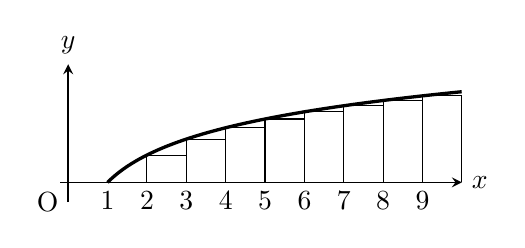
\begin{tikzpicture}[scale=0.5]
       \coordinate[label=below left:O](O)at(0,0);%原点O
       \coordinate(XS)at(-0.2,0);%x軸最小
       \coordinate(XL)at(10,0);%x軸最大
       \coordinate(YS)at(0,-0.5);%y軸最小
       \coordinate(YL)at(0,3);%y軸最大
       \draw[semithick,->,>=stealth](XS)--(XL)node[right]{$x$};%x軸
       \draw[semithick,->,>=stealth](YS)--(YL)node[above]{$y$};%y軸

       \foreach \t in{1,...,9}
           \draw(\t,0)node[below]{\t};%点 1-9

       \draw[very thick,samples=1000,domain=1:10]
           plot({\x},{ln(\x)});%対数

       \foreach \t in{2,...,9}
           \draw(\t,0)--(\t,{ln(\t)})
       --(\t+1,{ln(\t)})--(\t+1,0); %x=t,x=t+1の間の短冊

      \end{tikzpicture}
%
      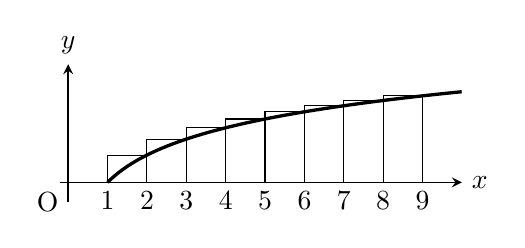
\begin{tikzpicture}[scale=0.5]
       \coordinate[label=below left:O](O)at(0,0);%原点O
       \coordinate(XS)at(-0.2,0);%x軸最小
       \coordinate(XL)at(10,0);%x軸最大
       \coordinate(YS)at(0,-0.5);%y軸最小
       \coordinate(YL)at(0,3);%y軸最大
       \draw[semithick,->,>=stealth](XS)--(XL)node[right]{$x$};%x軸
       \draw[semithick,->,>=stealth](YS)--(YL)node[above]{$y$};%y軸

       \foreach \t in{1,...,9}
           \draw(\t,0)node[below]{\t};%点 1-9

       \draw[very thick,samples=1000,domain=1:10]
           plot({\x},{ln(\x)});%対数

       \foreach \t in{2,...,9}
           \draw(\t,0)--(\t,{ln(\t)})
       --(\t-1,{ln(\t)})--(\t-1,0); %x=t,x=t+1の間の短冊

      \end{tikzpicture}


      そこで、
      左のグラフより次が得られる。
      \begin{align}
       \sum_{n=2}^{[x]}((n+1)-n)\log{n}
        <& \int_{1}^{[x]}\log{t}dt + \log{x}
        \leq \int_{1}^{x}\log{t}dt + \log{x}\\
        =& x\log{x}-x +1 +\log{x}
      \end{align}

      右のグラフより
      \begin{align}
       \sum_{n=2}^{[x]}(n-(n-1))\log{n}
        >& \int_{1}^{[x]}\log{t}dt
        \geq \int_{1}^{x}\log{t}dt -\log{x}\\
        =& x\log{x}-x +1  -\log{x}
      \end{align}

      これにより次の不等式を得る。
      \begin{equation}
       x\log{x}-x +1 -\log{x}
        \leq
        \sum_{n\leq x}\log{n}
        \leq
        x\log{x}-x +1 +\log{x}
      \end{equation}

      次のようにおく。
      \begin{equation}
       \sum_{n\leq x}\log{n} =
       x\log{x} - x + R(x)
      \end{equation}

      これにより
      \begin{equation}
       1 -\log{x}
        \leq
        R(x)
        \leq
        1 +\log{x}
      \end{equation}
      となり、
      $\lvert R(x) \rvert \leq 1+\log{x}$
      となる。


      \hrulefill
 \item
      ある定数$c$と関数$R:[1,+\infty) \to \mathbb{R}$が存在して、
      実数$x\geq 1$に対して、次が成立することを示せ。
      \begin{equation}
       \sum_{n\leq x} \frac{1}{\sqrt{n}}
        = 2\sqrt{x}+c +R(x)
        \quad \text{かつ}\quad
        \lvert R(x) \rvert \leq \frac{1}{\sqrt{x}}
      \end{equation}

      \dotfill

      
      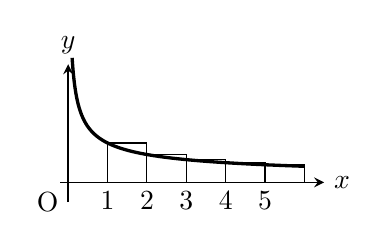
\begin{tikzpicture}[scale=0.5]
       \coordinate[label=below left:O](O)at(0,0);%原点O
       \coordinate(XS)at(-0.2,0);%x軸最小
       \coordinate(XL)at(6.5,0);%x軸最大
       \coordinate(YS)at(0,-0.5);%y軸最小
       \coordinate(YL)at(0,3);%y軸最大
       \draw[semithick,->,>=stealth](XS)--(XL)node[right]{$x$};%x軸
       \draw[semithick,->,>=stealth](YS)--(YL)node[above]{$y$};%y軸

       \foreach \t in{1,...,5}
           \draw(\t,0)node[below]{\t};%点 1-9

       \draw[very thick,samples=1000,domain=0.1:6]
           plot({\x},{1/sqrt(\x)});%根号

       \foreach \t in{1,...,5}
           \draw(\t,0)--(\t,{1/sqrt(\t)})
       --(\t+1,{1/sqrt(\t)})--(\t+1,0); %x=t,x=t+1の間の短冊

      \end{tikzpicture}
      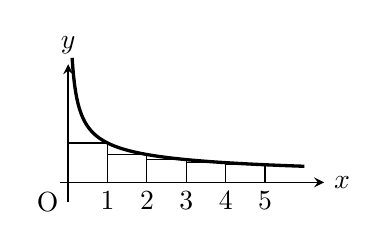
\begin{tikzpicture}[scale=0.5]
       \coordinate[label=below left:O](O)at(0,0);%原点O
       \coordinate(XS)at(-0.2,0);%x軸最小
       \coordinate(XL)at(6.5,0);%x軸最大
       \coordinate(YS)at(0,-0.5);%y軸最小
       \coordinate(YL)at(0,3);%y軸最大
       \draw[semithick,->,>=stealth](XS)--(XL)node[right]{$x$};%x軸
       \draw[semithick,->,>=stealth](YS)--(YL)node[above]{$y$};%y軸

       \foreach \t in{1,...,5}
           \draw(\t,0)node[below]{\t};%点 1-9

       \draw[very thick,samples=1000,domain=0.1:6]
           plot({\x},{1/sqrt(\x)});%根号

       \foreach \t in{1,...,5}
           \draw(\t,0)--(\t,{1/sqrt(\t)})
       --(\t-1,{1/sqrt(\t)})--(\t-1,0); %x=t,x=t+1の間の短冊

      \end{tikzpicture}


      \begin{equation}
       \int_{1}^{x} \frac{1}{\sqrt{t}}dt
        +(1-\{x\})\frac{1}{\sqrt{x}}
        <
       \sum_{n \leq x} \frac{1}{\sqrt{x}}
        <
        1 + \int_{1}^{x} \frac{1}{\sqrt{t}}dt
        -\{x\}\frac{1}{\sqrt{x}}
      \end{equation}

      \begin{align}
       \sum_{n \leq x} \frac{1}{\sqrt{x}}
        <&
        1 + \int_{1}^{x} \frac{1}{\sqrt{t}}dt
        -\{x\}\frac{1}{\sqrt{x}}
       < 1 + \int_{1}^{x} \frac{1}{\sqrt{t}}dt +\frac{1}{\sqrt{x}}\\
       \sum_{n \leq x} \frac{1}{\sqrt{x}}
       >&
       \int_{1}^{x} \frac{1}{\sqrt{t}}dt +(1-\{x\})\frac{1}{\sqrt{x}}
       > \int_{1}^{x} \frac{1}{\sqrt{t}}dt -\frac{1}{\sqrt{x}}
      \end{align}


      \begin{equation}
       \sum_{n \leq x} \frac{1}{\sqrt{x}}
        = \int_{1}^{x} \frac{1}{\sqrt{t}}dt
        +R(x)
      \end{equation}
      とおくと
      \begin{equation}
       -\frac{1}{\sqrt{x}}
        <
       R(x)
        <
        1+\frac{1}{\sqrt{x}}
      \end{equation}






      \hrulefill
 \item
      ある定数$c$と関数$R:[1,+\infty) \to \mathbb{R}$が存在して、
      実数$x\geq e$に対して、次が成立することを示せ。
      \begin{equation}
       \sum_{n\leq x} \frac{\log{n}}{n}
        = \frac{1}{2}(\log{x})^2 +c+R(x)
        \quad \text{かつ}\quad
        \lvert R(x) \rvert \leq \frac{\log{x}}{x}
      \end{equation}

      \dotfill
      

      関数$y=\frac{\log{x}}{x}$は
      $x\geq e$において単調減少である。

      \begin{equation}
       \sum_{n\leq x} \frac{\log{n}}{n}
        = \frac{\log{2}}{2}
        + \sum_{n=3}^{[x]} \frac{\log{n}}{n}
      \end{equation}

      \begin{equation}
       \int_{3}^{x} \frac{\log{t}}{t}dt
        +
        (1-\{x\})\frac{\log{x}}{x}
       <
       \sum_{n=3}^{[x]} \frac{\log{n}}{n}
       <
       \frac{\log{3}}{3}
       + \int_{3}^{x} \frac{\log{t}}{t}dt
       - \{x\}\frac{\log{x}}{x}
      \end{equation}


      \begin{equation}
       \sum_{n\leq x} \frac{\log{n}}{n}
        = \frac{\log{2}}{2} + \int_{3}^{x} \frac{\log{t}}{t}dt +R(x)
      \end{equation}
      とすると、
      \begin{equation}
        (1-\{x\})\frac{\log{x}}{x}
       <
       R(x)
       <
       \frac{\log{3}}{3}
       - \{x\}\frac{\log{x}}{x}
      \end{equation}
      

      
      

      \hrulefill
 \item
      実数$x,k\geq 1$に対して、次を示せ。
      \begin{equation}
       \sum_{n\leq x}\left( \log{\frac{x}{n}} \right)^k \leq k! x
      \end{equation}

      (ヒント:微分積分学の基本定理を
      \begin{equation}
       \left( \log{\frac{x}{n}} \right)^{k}
        = k\int_{1}^{\frac{x}{n}} \frac{(\log{u})^{k-1}}{u} \mathrm{d}u
      \end{equation}
      という形で用いる。
      )


\end{enumerate}


\hrulefill

\end{document}
